\begin{figure}[ht]
		\centering
		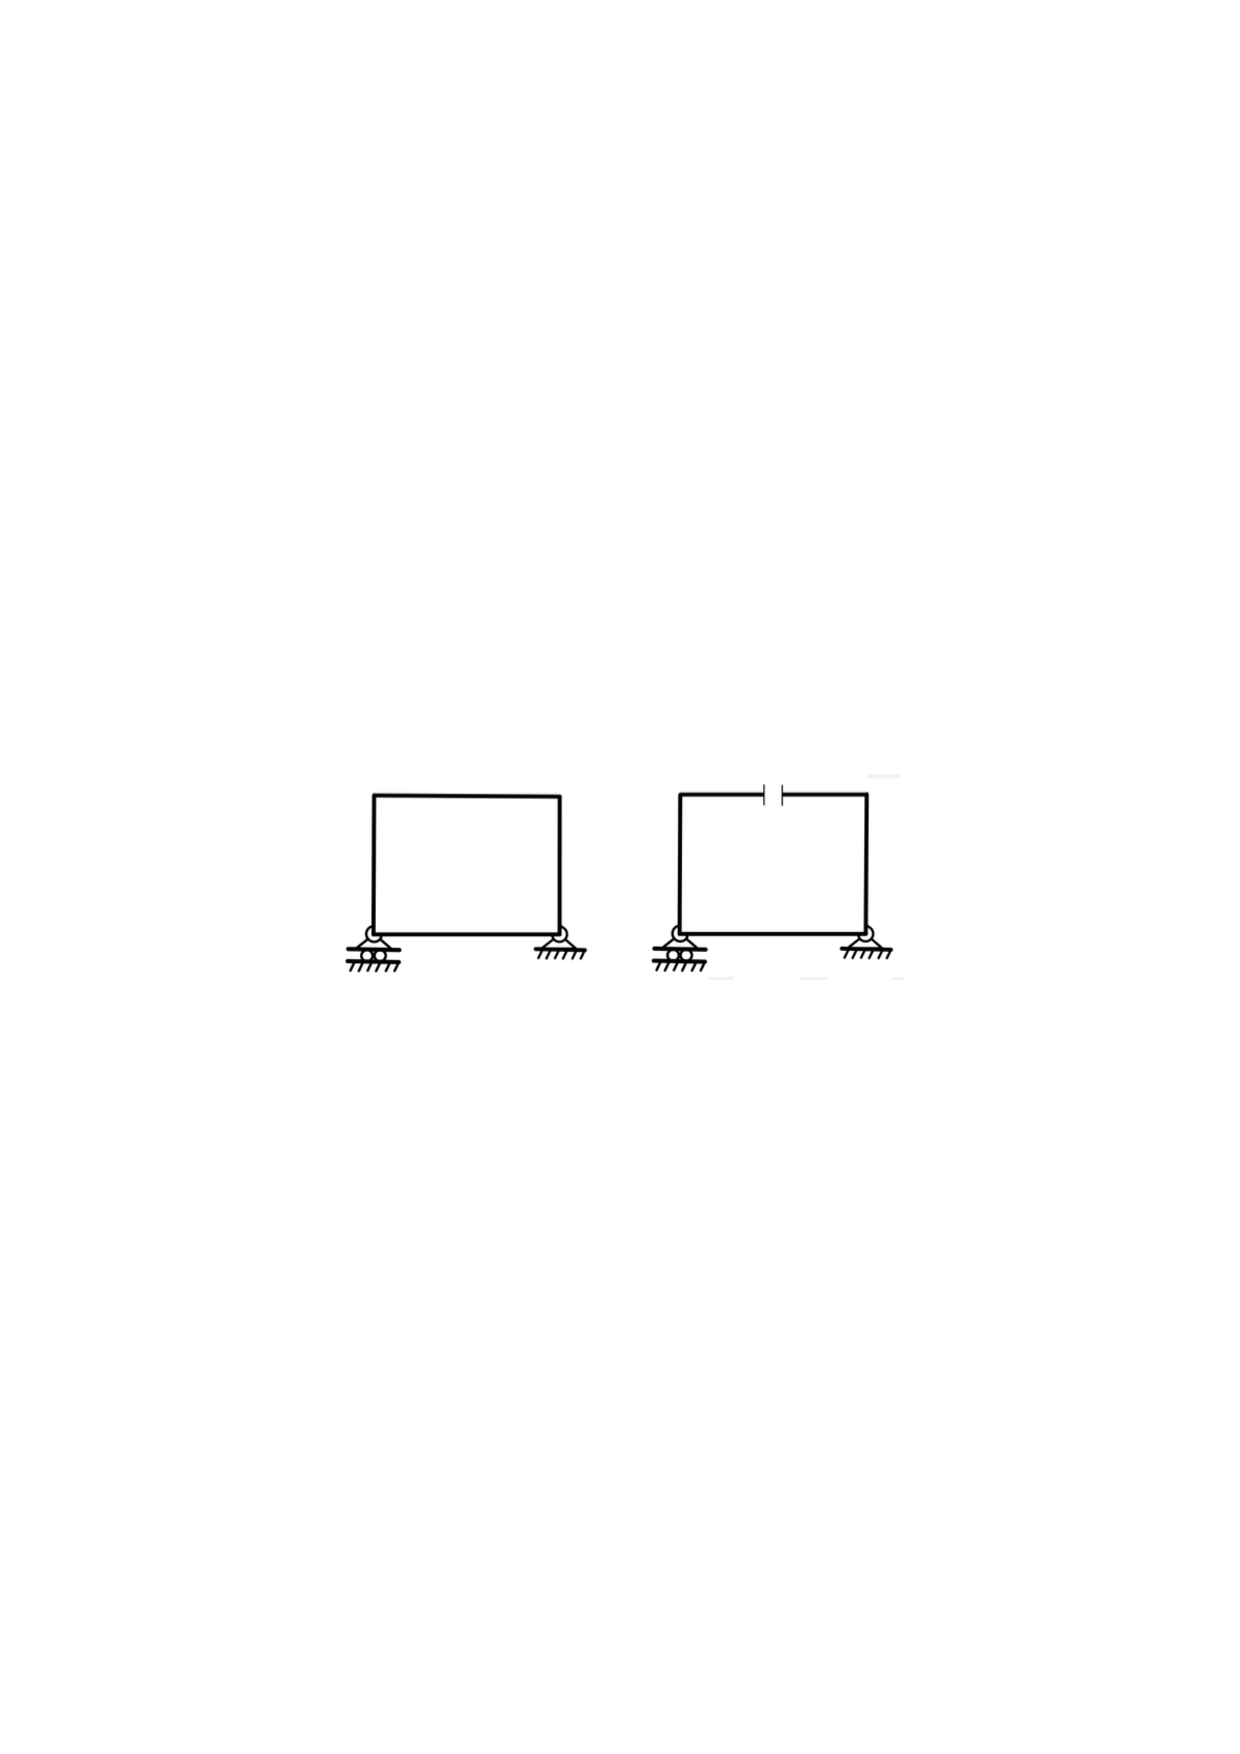
\includegraphics[scale=0.75]{cin_apertifinti.pdf}
		\caption{Portale rettangolare (schema ripreso nel
			Vol.~II per il caso deformabile): maglia chiusa
			(sinistra, $\nu = -3$) e maglia aperta con
			taglio completo nella traversa superiore
			(destra, $\nu = 0$). Il taglio rimuove
			esattamente $3(p-1) = 3$ gradi di iperstaticità.}
		\label{fig:portale_biconnesso}
	\end{figure}
